\begin{titlepage}
    \begin{center}

        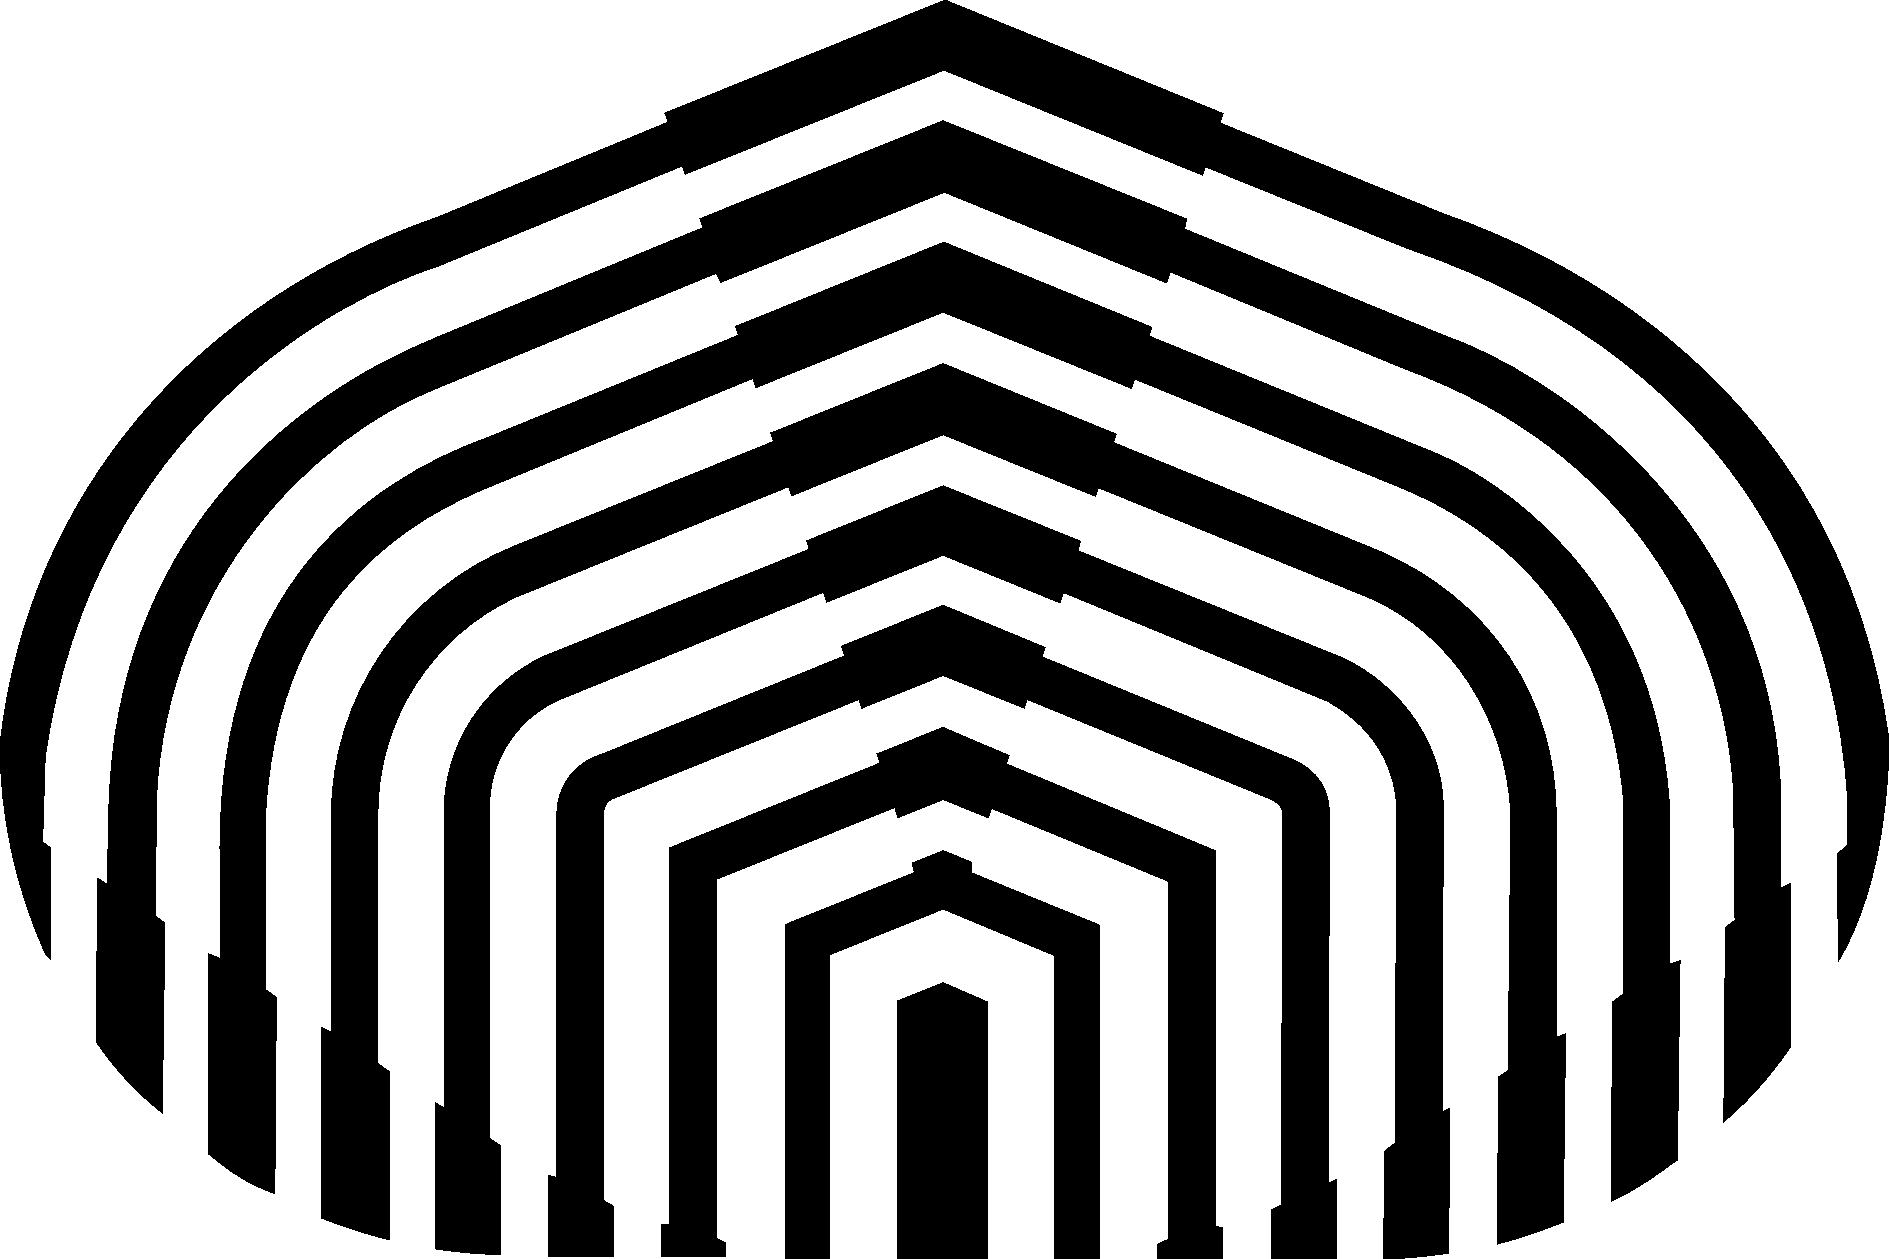
\includegraphics[scale=0.5]{usb.png} \\
        \textsc {\large UNIVERSIDAD SIMÓN BOLÍVAR} \\
        \textsc{DECANATO DE ESTUDIOS PROFESIONALES\\
        COORDINACIÓN DE INGENIERÍA ELECTRÓNICA}\\
        \textbf{SISTEMA DE GENERACIÓN DE MOSAICOS 2D PARA ROBOTS MÓVILES A PARTIR DE VIDEO MONOCULAR} \\
        PROYECTO DE GRADO \\
        PRESENTADO POR: \\
        Victor Yovanni Garcia Carmona, Carnet: 12-10738

    \end{center}
% El resumen debe ser de una sola página
\addtotoc{Resumen}
\abstract
{
    \addtocontents{toc}{\vspace{1em}}
    Al realizar tareas de exploración para el análisis del suelo desde espacios aereos o del fondo marino, es muy comun emplear sistemas de adquisición basados en captura de videos para su posterior análisis. En la actualidad, el incremento de la tecnologia sobre el procesamiento de datos, ha permitido que los algoritmos de vision por computadora coloquen a la camara como principal sensor para la reconstruccion de entornos recorridos por vehiculos móviles. El presente trabajo se encuantra enfocado al analisis y la implementación de distintos algoritmos para la reconstrucción de un mosaico 2D (dos dimensiones), a partir de la información proveniente de una camara monocular ubicada en la parte inferior de un robot. El robot en cuestión puede realizar recorridos aereos para realizar la adquisición del video, o incluso trayectorias mas desafiantes como serian las aplicaciones subacuaticas. Para esto, se implementarán distintos algoritmos usando tecnicas de procesamiento de imagenes y vision por computadora, para la elaboracion de un sistema automatizado que permita generar un mapa en dos dimensiones de la trayectoria recorrida, con la menor distorsion posible, mejorando la detección de puntos clave, y optimizando el calculo de las matrices de transformación para la alineación de imagenes en el mosaico, ademas de realizar analisis sobre el error de reproyeccion de dichas imagenes en el mapa del suelo generado.
    
}

% Las palabras clave son generalmente los nombres de áreas de investigación a
% los cuales está asociado el trabajo. Generalmente son tres o cuatro.
\noindent \begin{small} \textbf{Palabras clave}: mosaico, video monocular, puntos clave, matriz de transformación. 
\end{small}
	
% Iniciar nueva página luego del resumen
\clearpage
\setstretch{1.3}

\end{titlepage}